\documentclass[11pt]{article}

\usepackage[margin=1in]{geometry}
\usepackage{amsmath,amssymb,amsfonts,amsthm,bm,mathtools}
\usepackage{graphicx}
\usepackage{booktabs}
\usepackage{subcaption}
\usepackage{enumitem}
\usepackage{hyperref}
\usepackage[numbers,sort&compress]{natbib}
\usepackage{xcolor}
\usepackage{microtype}
\usepackage{algorithm}
\usepackage{algorithmic}

\graphicspath{{figures/}}

\newcommand{\R}{\mathcal{R}}
\newcommand{\Pcal}{\mathcal{P}}
\newcommand{\Sset}{\mathcal{S}}
\newcommand{\Znn}{\mathbb{Z}_{\ge 0}}
\newcommand{\E}{\mathbb{E}}
\newcommand{\Bin}{\operatorname{Bin}}
\newcommand{\TV}{\operatorname{TV}}
\newcommand{\RDME}{\operatorname{RDME}}
\newcommand{\CME}{\operatorname{CME}}
\newcommand{\diag}{\operatorname{diag}}

\newtheorem{proposition}{Proposition}
\newtheorem{remark}{Remark}

\title{A Two-Level Multigrid Method for the\\
Reaction--Diffusion Master Equation}
\author{Aditya Dendukuri}
\date{}

\begin{document}
\maketitle

\begin{abstract}
We develop a two-level multigrid finite state projection (FSP) method for the
reaction--diffusion master equation (RDME). The central observation is that
pairwise voxel aggregation is a Kemeny--Snell lumping of the Markov chain
generated by fast intra-pair diffusion. This yields a coarse generator of the
Galerkin form $\bar A = \R A \Pcal$, where restriction is exact marginalization
and prolongation is induced by the local stationary law of the fast diffusion
operator. For pair aggregation, this prolongation is Binomial.

The multigrid cycle uses intra-pair diffusion as the smoother, exact restriction
to transfer the pre-smoothed distribution to the coarse level, a coarse RDME
solve, and prolongation of the coarse \emph{correction} $\delta^{2h} = \tilde
p^{2h} - p^{2h}$ back to the fine level.  This is a full-approximation
scheme (FAS) for the probability generator.  The coarse generator is exact for
linear birth--death--diffusion systems and provides a tractable closure for
nonlinear reaction networks.

Uniform coarsening fails at bistable interfaces because the Binomial
prolongation cannot distinguish the two orientations of an interface pair.
This motivates an adaptive extension in which the refinement criterion, based on
within-pair asymmetry, inter-pair gradient, and per-molecule flux diagnostics,
localizes coarsening to homogeneous bulk regions.  Fine and coarse pairs are
then co-evolved in a persistent mixed-resolution FSP that avoids rematerializing
the full fine grid.

Numerical experiments on one-dimensional birth--death and Schl\"ogl
reaction--diffusion systems demonstrate: (i)~exact coarse evolution for linear
networks; (ii)~V-cycle accuracy on nonlinear bistable fronts with measurable
stiffness reduction; (iii)~automatic front localization and persistent
mixed-resolution evolution; (iv)~second-level quad-coarsening with policy
verification that bulk-only promotion is enforced. These results establish
adaptive multigrid FSP as a distribution-resolving method for low-copy spatial
systems with localized metastable structure.
\end{abstract}

\section{Introduction}

The reaction--diffusion master equation (RDME) provides a mesoscopic Markov
description of spatial stochastic chemical kinetics by coupling local reaction
channels with diffusive transport between neighboring voxels
\citep{Gillespie1977,Erban2009}. When the underlying process is low-copy,
multimodal, or metastable, the full probability distribution may be the object
of interest rather than only moments or sample paths. Finite state projection
(FSP) methods are attractive in this regime because they approximate the
chemical master equation directly on a truncated state space with explicit mass
control \citep{Munsky2006}. The difficulty is that spatial discretization makes
the state space grow rapidly with the number of voxels, while diffusion
introduces fast modes that aggravate stiffness.

This paper develops a multigrid reduction strategy for the RDME that targets
the spatial dimension directly. The basic coarsening step merges adjacent
voxels into pairs and formulates the resulting operator as a genuine
Galerkin coarse generator. At the algorithmic level, this yields a two-level
FAS-style V-cycle:
\begin{enumerate}[itemsep=0.2em]
  \item \textbf{Pre-smooth}: evolve the fast intra-pair diffusion modes to drive
    within-pair distributions toward the local equilibrium (Binomial for
    identical voxels).
  \item \textbf{Restrict}: marginalize onto pair totals.
  \item \textbf{Coarse solve}: advance the coarse RDME.
  \item \textbf{Correct}: prolong the coarse correction
    $\delta^{2h} = \tilde p^{2h} - p^{2h}$ to the fine level.
  \item \textbf{Post-smooth}: re-equilibrate within-pair distributions.
\end{enumerate}
Only the correction $\delta^{2h}$, not the full coarse distribution, is
prolongated. This keeps the fine state space small: it grows only from the
fraction of probability that moves during the coarse solve, not from the entire
coarse support.

For linear birth--death--diffusion systems, the coarse operator closes exactly.
For nonlinear systems such as the Schl\"ogl model, Binomial within-pair
equilibration gives explicit coarse propensities. The V-cycle is accurate in
homogeneous bulk but fails at bistable interfaces, where the fine conditional
distribution deviates sharply from Binomial. This failure mode leads naturally
to an adaptive strategy: coarsen only where the local distribution is
redundant, and retain fine resolution where the interface structure matters.

The adaptive extension is a persistent mixed-resolution FSP: fine and coarse
pairs are co-evolved on a single mixed-resolution state space, the refinement
region is updated adaptively, and the full fine grid is never materialized.
Second-level quad-coarsening (merging two pair-coarse voxels) extends the
hierarchy one level further, with a policy validation confirming that the
adaptive criterion keeps this aggressive coarsening confined to spatially
distant bulk pairs.

The language of restriction and prolongation is classical multigrid
\citep{Briggs2000,Trottenberg2001}, but the reduced operator is a probability
generator rather than an elliptic discretization, and the prolongation is
probabilistic rather than interpolatory. The present manuscript is focused on
the one-dimensional single-species case to expose the main ideas clearly.
Within that scope, the contributions are as follows.
\begin{enumerate}[itemsep=0.2em]
  \item We formulate pairwise spatial coarsening as a Kemeny--Snell
    aggregation of the RDME Markov chain \citep{kemeny_snell_1960,Buchholz1994}
    and derive the exact Galerkin coarse generator.
  \item We construct a two-level FAS-style V-cycle for the probability
    generator, prove exactness for linear networks, and characterize the
    Binomial closure used in nonlinear coarse propensities.
  \item We identify the interface failure mode of uniform coarsening and
    introduce an adaptive mixed-resolution strategy that avoids coarsening
    such regions.
  \item We validate second-level quad-coarsening on a twelve-voxel domain,
    including a policy audit showing that the adaptive criterion protects
    front-adjacent pairs from quad coarsening.
\end{enumerate}

The intended regime is not large-scale bulk simulation, where
trajectory-based methods remain more practical, but low-count spatial systems
for which the distribution itself matters: interfaces, rare switching events,
and localized metastable structures.

\section{RDME and spatial aggregation}

\subsection{Fine-grid RDME}

Let a one-dimensional domain be partitioned into $K$ voxels of width $h$, and
let
\[
  \bm{x}=(n_1,\dots,n_K)\in\Znn^K
\]
denote the vector of molecule counts. The RDME defines a continuous-time Markov
chain on $\Znn^K$ with generator
\[
  A = A_{\mathrm{rxn}} + A_{\mathrm{diff}}.
\]
The reaction part acts independently within each voxel, while the diffusion
part transports molecules between neighboring voxels at rate $d=D/h^2$.

Given a truncated state space $\Sset_h \subset \Znn^K$, FSP replaces the full
generator by its restriction to $\Sset_h$ and evolves the projected
distribution by matrix exponentiation \citep{Munsky2006}. In spatial problems,
the size of $\Sset_h$ grows rapidly with $K$, and the fine-grid diffusion rate
$d=D/h^2$ becomes large as $h\to 0$.

\subsection{Pair aggregation as a Markov-chain lumping}

Assume $K$ is even and partition the fine grid into voxel pairs
$\{1,2\},\{3,4\},\dots,\{K-1,K\}$.
Define the coarse variables
\[
  \bar n_j = n_{2j-1}+n_{2j}, \qquad j=1,\dots,K/2,
\]
and let $\bar{\bm{x}}=(\bar n_1,\dots,\bar n_{K/2})$.
Restriction is exact marginalization over within-pair splits:
\[
  (\R p)(\bar{\bm{x}})
  = \sum_{\bm{x}:\, n_{2j-1}+n_{2j}=\bar n_j\ \forall j} p(\bm{x}).
\]

When intra-pair diffusion equilibrates rapidly relative to the remaining
dynamics, the fine states compatible with the same $\bar{\bm{x}}$ mix toward a
local stationary law. For identical neighboring subvoxels this law is
Binomial:
\[
  \pi(m\mid \bar n_j)=\Bin(\bar n_j,\tfrac12)(m),
  \qquad m=0,\dots,\bar n_j.
\]
The prolongation operator is the product of within-pair conditional laws,
\[
  (\Pcal \bar p)(\bm{x})
  = \bar p(\bar{\bm{x}})\prod_{j=1}^{K/2} \pi(n_{2j-1}\mid \bar n_j),
\]
and the coarse generator is
\[
  \bar A = \R A \Pcal.
\]
This is the standard Kemeny--Snell form for aggregation of a Markov chain by
fast local equilibration \citep{kemeny_snell_1960,Buchholz1994,Simon1961}.

\begin{remark}
The same operator template appears in quasi-steady-state reductions of
well-mixed stochastic reaction networks, where fast reaction subnetworks are
collapsed and the prolongation is defined by a local invariant distribution
\citep{peles,CAO20083472,Cao2016}. In the present setting, the fast process is
spatial diffusion rather than a fast reaction subsystem.
\end{remark}

\section{Two-level FAS-style V-cycle}
\label{sec:vcycle}

\subsection{Algorithm}

Algorithm~\ref{alg:vcycle} states the two-level cycle precisely.
The key design choices are:
\begin{itemize}[itemsep=0.2em]
  \item \textbf{Smoother}: intra-pair diffusion only. This drives within-pair
    distributions toward the Binomial equilibrium $\pi(\cdot\mid \bar n_j)$
    without perturbing the pair totals $\bar n_j$. It is a
    genuine smoother for the fast spatial modes introduced by fine-grid
    diffusion.
  \item \textbf{Correction, not substitution}: only the coarse correction
    $\delta^{2h} = \tilde p^{2h} - p^{2h}$ is prolongated and added to the
    pre-smoothed fine distribution. The fine state space grows only from the
    probability that moved during the coarse solve, not from the entire coarse
    support. This is the Full Approximation Scheme (FAS) applied to the
    probability generator.
  \item \textbf{Signed prolongation}: $\delta^{2h}$ is signed. To apply the
    (non-negative) prolongation operator, positive and negative parts are
    prolongated separately and then combined. Small numerically-negative
    probabilities arising from cancellation are clipped to zero.
\end{itemize}

\begin{algorithm}[t]
\caption{Two-level FAS V-cycle for the RDME}
\label{alg:vcycle}
\begin{algorithmic}[1]
\REQUIRE Fine distribution $p^h$, time step $\Delta t$, smoothing times $\tau_{\rm pre}, \tau_{\rm post}$
\STATE \textbf{Pre-smooth}: $\tilde p^h \leftarrow e^{A_{\rm intra}\,\tau_{\rm pre}} p^h$
  \hfill \COMMENT{intra-pair diffusion only}
\STATE \textbf{Restrict}: $p^{2h} \leftarrow \R\,\tilde p^h$
\STATE \textbf{Coarse expand}: add FSP boundary shells to $\Sset_{2h}$
\STATE \textbf{Coarse solve}: $\tilde p^{2h} \leftarrow e^{\bar A\,\Delta t}\,p^{2h}$
\STATE \textbf{Correction}: $\delta^{2h} \leftarrow \tilde p^{2h} - p^{2h}$
\STATE \textbf{Prolong correction}: $p^h_{\rm new} \leftarrow \tilde p^h + \Pcal\,\delta^{2h}$
\STATE \textbf{Post-smooth}: $p^h_{\rm new} \leftarrow e^{A_{\rm intra}\,\tau_{\rm post}} p^h_{\rm new}$
\ENSURE Updated fine distribution $p^h_{\rm new}$
\end{algorithmic}
\end{algorithm}

\subsection{Coarse operators and closure}

\subsubsection{Linear birth--death--diffusion systems}

Consider a one-species birth--death--diffusion model with per-voxel reactions
$\varnothing \xrightarrow{k_b} A$ and $A \xrightarrow{k_d} \varnothing$,
and nearest-neighbor diffusion. Under pair aggregation:
\begin{itemize}[itemsep=0.15em]
  \item the coarse diffusion rate is $D/(2h)^2 = d/4$;
  \item the coarse birth rate doubles (one coarse voxel represents two fine
        voxels);
  \item the death rate remains first-order in the coarse count.
\end{itemize}
Since the generator is linear in the state, the aggregated operator closes
exactly.

\begin{proposition}
For the one-dimensional birth--death--diffusion RDME with pairwise spatial
aggregation and Binomial prolongation, the Galerkin coarse generator
$\bar A = \R A \Pcal$ coincides with the exact RDME generator on the $K/2$-voxel
coarse grid.
\end{proposition}

Figure~\ref{fig:birthdeath} confirms this numerically: the coarse and fine
solutions are indistinguishable at the distribution level while the coarse
state space is dramatically smaller.

\begin{figure}[t]
  \centering
  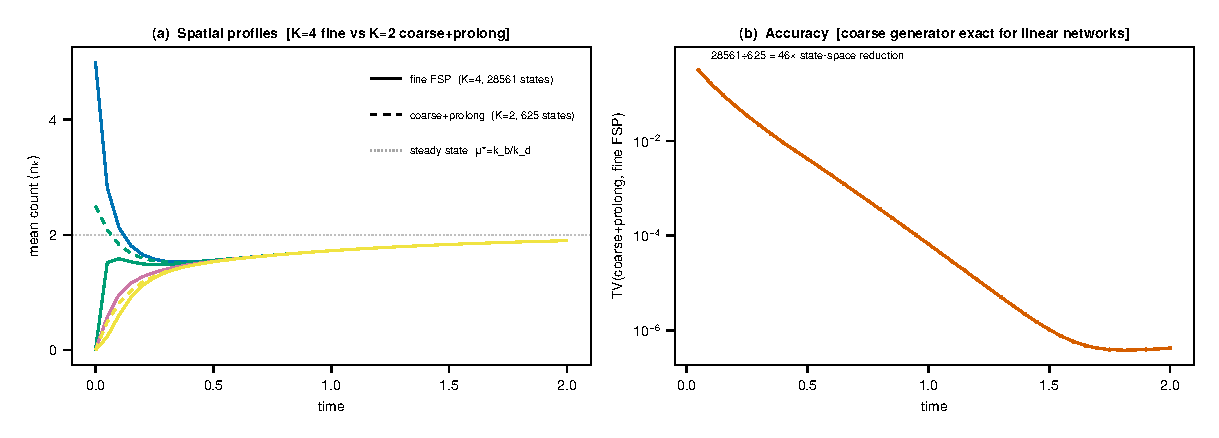
\includegraphics[width=\textwidth]{fig_birthdeath}
  \caption{Linear birth--death--diffusion benchmark. The pair-aggregated coarse
  generator is exact for this linear system, and the coarse solution prolonged
  to the fine grid matches the fine FSP solution while using far fewer states.}
  \label{fig:birthdeath}
\end{figure}

\subsubsection{Nonlinear Schl\"ogl closure}

We use the one-dimensional Schl\"ogl model as the canonical nonlinear test
problem. In each voxel,
\[
  \varnothing \xrightarrow{c_3} X,\qquad
  X \xrightarrow{c_4} \varnothing,\qquad
  2X \xrightarrow{c_1} 3X,\qquad
  3X \xrightarrow{c_2} 2X.
\]
The coarse zeroth- and first-order propensities remain exact under pair
aggregation. The autocatalytic and reverse reactions require conditional
moments of the within-pair split; under the Binomial model
$n_{2j-1}\mid \bar n_j \sim \Bin(\bar n_j,\tfrac12)$:
\begin{align*}
  a_{\mathrm{auto}}^{\mathrm{coarse}}(\bar n_j)
    &= c_1\,\frac{\bar n_j(\bar n_j-1)}{4}, \\
  a_{\mathrm{rev}}^{\mathrm{coarse}}(\bar n_j)
    &= c_2\,\frac{\bar n_j(\bar n_j-1)(\bar n_j-2)}{24}.
\end{align*}

The closure is accurate when the within-pair conditional is close to the
fast-diffusion equilibrium. Figure~\ref{fig:closure} compares exact conditional
factorial moments from a fine FSP solution against the Binomial predictions: a
bulk pair is near symmetric equilibrium with small closure error, while an
interface pair is highly asymmetric and the closure error is order-one.

\begin{figure}[t]
  \centering
  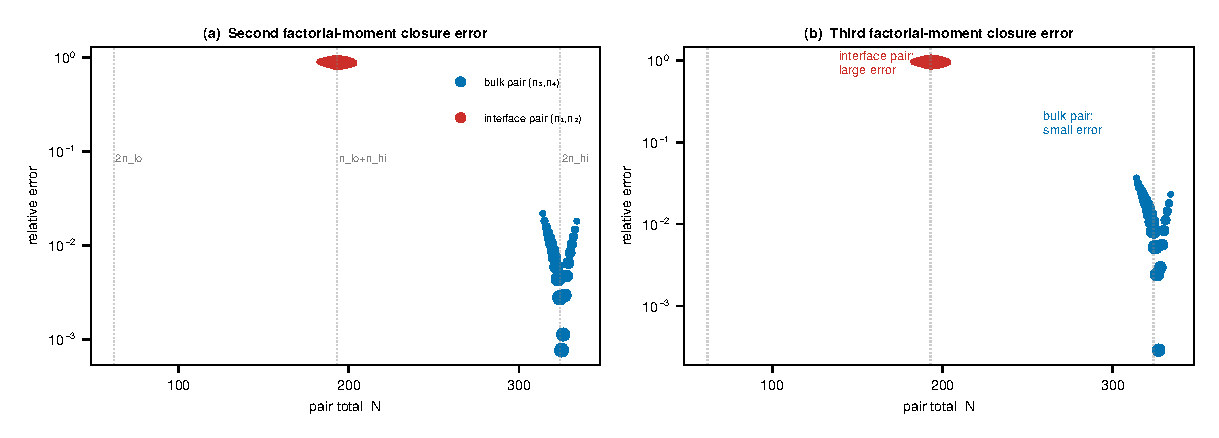
\includegraphics[width=\textwidth]{fig_closure}
  \caption{Conditional-moment closure for the Schl\"ogl model. Binomial closure
  is accurate for a homogeneous bulk pair but fails sharply at a bistable
  interface. This is the structural reason the V-cycle and the adaptive method
  retain interface pairs at fine resolution.}
  \label{fig:closure}
\end{figure}

\section{V-cycle results: nonlinear Schl\"ogl front}
\label{sec:vcycle_results}

Figure~\ref{fig:vcycle_means} shows the V-cycle applied to the Schl\"ogl
model on an eight-voxel grid with a bistable front initial condition.
Voxel means from the V-cycle solution are compared against a direct fine-grid
FSP reference. The V-cycle tracks the reference accurately: the front position
and amplitude are captured without materializing the full fine-grid state space
at each step.

\begin{figure}[t]
  \centering
  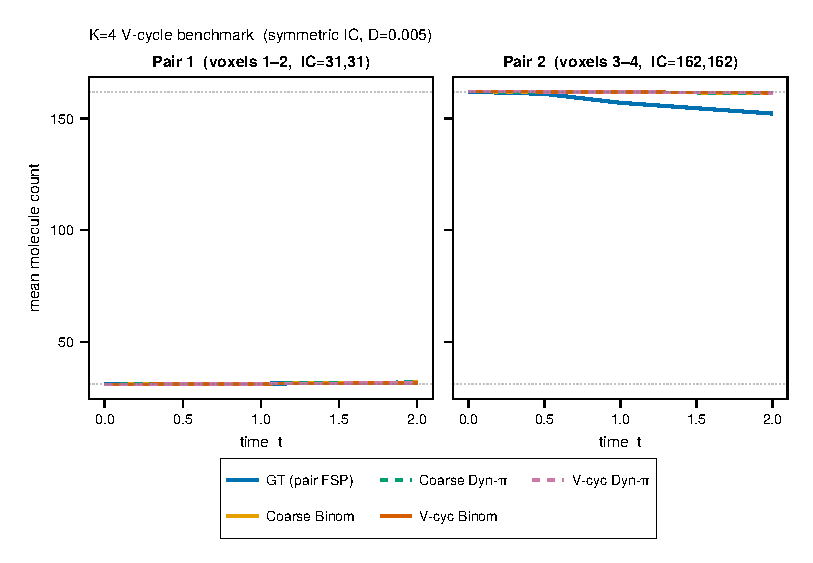
\includegraphics[width=\textwidth]{fig5_vcycle_means}
  \caption{V-cycle voxel means versus fine FSP reference on the $K=8$
  Schl\"ogl bistable front. The two-level FAS cycle tracks the reference
  spatial profile accurately throughout the evolution.}
  \label{fig:vcycle_means}
\end{figure}

Figure~\ref{fig:vcycle_accuracy} quantifies accuracy more precisely.
Total variation distance between the V-cycle prolongated distribution and the
fine reference is small and stable, confirming that the coarse correction
mechanism is propagating the relevant fine-level information faithfully.
Figure~\ref{fig:stiffness} shows the stiffness reduction: coarsening replaces
the fine diffusion rate $D/h^2$ by $D/(2h)^2$, doubling the largest accepted
time step at fixed distribution error.

\begin{figure}[t]
  \centering
  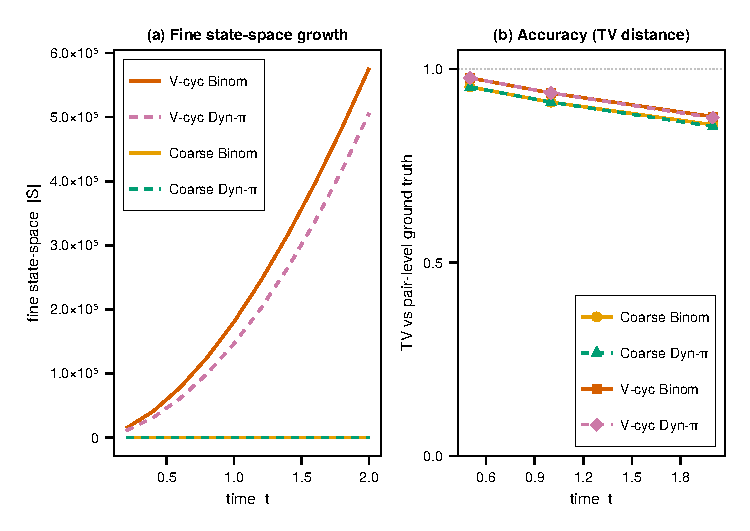
\includegraphics[width=\textwidth]{fig6_vcycle_accuracy}
  \caption{V-cycle accuracy on the $K=8$ Schl\"ogl front. Total variation
  distance between the V-cycle prolongated distribution and the direct fine FSP
  reference remains small throughout the run, confirming coarse correction
  quality.}
  \label{fig:vcycle_accuracy}
\end{figure}

\begin{figure}[t]
  \centering
  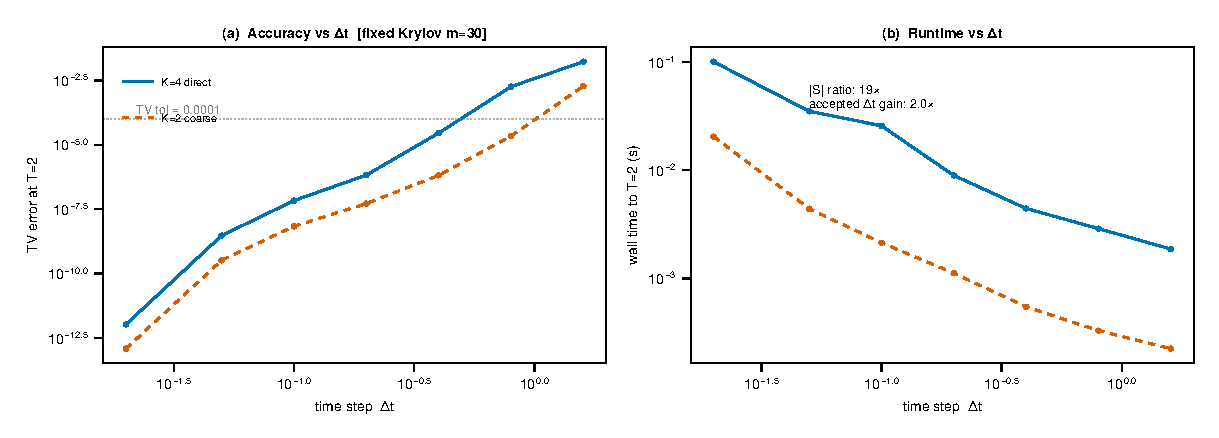
\includegraphics[width=\textwidth]{fig_stiffness}
  \caption{Empirical stiffness benchmark. Coarsening reduces the diffusion
  stiffness and permits larger accepted time steps at fixed distributional
  error.}
  \label{fig:stiffness}
\end{figure}

\section{Failure of uniform coarsening at fronts}
\label{sec:failure}

\subsection{The interface failure mode}

If an interface lies inside an aggregated pair, then the coarse variable
$\bar n_j$ loses the orientation of the front. In the Schl\"ogl front regime,
the two fine states $(n_{\ell},n_h)$ and $(n_h,n_{\ell})$ have the same coarse
sum $n_{\ell}+n_h$ but represent distinct spatial configurations. Uniform
coarsening therefore destroys exactly the information needed to resolve the
interface distribution.

\subsection{Refinement diagnostics}

The adaptive criterion combines three diagnostics defined from the current
distribution.
\begin{enumerate}[itemsep=0.25em]
  \item \textbf{Within-pair asymmetry}
  \[
    \alpha_j = \frac{|\mu_{2j-1}-\mu_{2j}|}{\mu_{2j-1}+\mu_{2j}},
    \qquad \mu_k=\E[n_k].
  \]

  \item \textbf{Inter-pair gradient}
  \[
    \beta_j = \frac{|\mu_{2j}-\mu_{2j+1}|}{\mu_{2j}+\mu_{2j+1}}.
  \]

  \item \textbf{Per-molecule flux}
  \[
    \varphi_j
    = \frac{d\,\mu_{2j-1}/\max(1,\mu_{2j-1})}
           {\bar\varphi_{\mathrm{domain}}},
  \]
  guarding low-count transport bottlenecks.
\end{enumerate}
The effective asymmetry for front detection is
\[
  \alpha_j^{\mathrm{eff}} = \max\{\alpha_j,\beta_{j-1},\beta_j\}.
\]
Hysteresis thresholds $(\alpha_{\mathrm{lo}},\alpha_{\mathrm{hi}})$ prevent
rapid mask oscillation. Figure~\ref{fig:criterion} illustrates three
representative scenarios: a front inside a pair, a front on a pair boundary,
and a homogeneous region.

\begin{figure}[t]
  \centering
  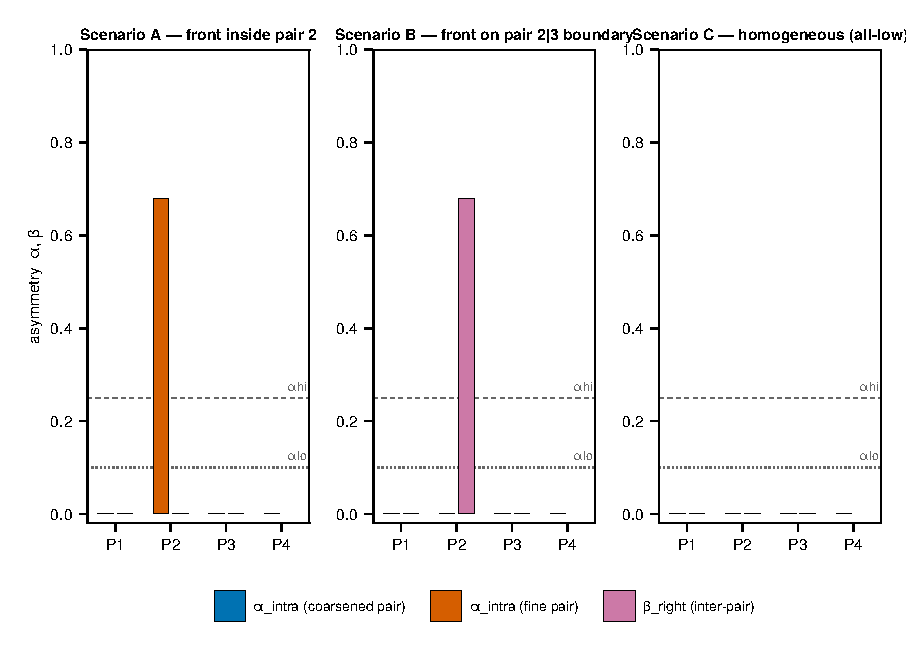
\includegraphics[width=\textwidth]{fig_adaptive_criterion}
  \caption{Adaptive refinement diagnostics on representative $K=8$ Schl\"ogl
  states. The within-pair asymmetry $\alpha$ detects fronts inside a pair,
  while the inter-pair gradient $\beta$ detects fronts aligned with a pair
  boundary.}
  \label{fig:criterion}
\end{figure}

\subsection{Localized refinement region}

Rather than allowing arbitrary disconnected fine pairs, we define a contiguous
refinement region. Pairs flagged by the criterion are collected, the smallest
interval containing them is formed, and an optional halo of neighboring pairs
is added. This localized refinement region is aligned with the spatial
structure of fronts and simplifies repartitioning.

\section{Adaptive mixed-resolution extension}
\label{sec:mixed}

\subsection{Mixed-resolution RDME}

Once the refinement region is selected, the state lives on a mixed-resolution
space $\Sset^M \subset \Znn^{K_M}$, where each fine pair contributes two
coordinates and each coarse pair contributes one. The mixed generator is
assembled directly:
\begin{itemize}[itemsep=0.2em]
  \item fine pairs use the original voxel-level reactions and intra-pair
        diffusion,
  \item coarse pairs use the Binomial-closed coarse propensities,
  \item cross-pair diffusion uses first-moment boundary closure when one side
        is coarse.
\end{itemize}
Interface pairs are never coarsened, so their within-pair distribution is never
approximated by a Binomial law.

\subsection{Persistent mixed-state evolution}

Rather than taking one mixed step and prolongating back to the full fine grid,
we evolve directly on the mixed-resolution state space:
\begin{enumerate}[itemsep=0.2em]
  \item evaluate the refinement criterion when required,
  \item update the partition only if the localized refinement region changes,
  \item adapt the current mixed state by pairwise marginalization or Binomial
        splitting,
  \item expand the mixed FSP state space,
  \item solve the mixed RDME over one time step,
  \item prune low-probability states.
\end{enumerate}
Fine-grid reconstruction is performed only when a fine observable is requested.
A pair-space center-of-mass triggers a full repartition only when the front
drifts past a threshold.

\subsection{Adaptive front resolution}

Figure~\ref{fig:adaptive_accuracy} compares direct FSP, uniform coarsening,
and adaptive coarsening on a $K=4$ Schl\"ogl front problem. The adaptive
method retains the front pair at fine resolution and coarsens the homogeneous
pair, reducing the approximation error substantially relative to uniform
coarsening. Figure~\ref{fig:adaptive_mask} shows the corresponding
time-dependent mask.

\begin{figure}[t]
  \centering
  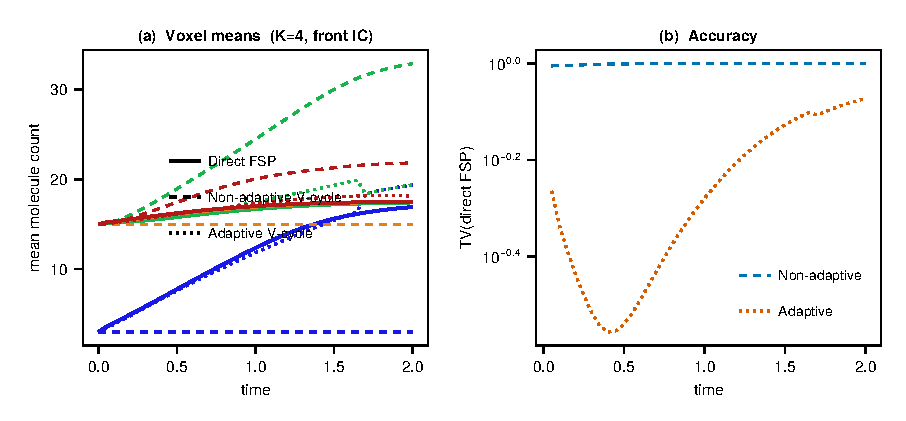
\includegraphics[width=\textwidth]{fig_adaptive_accuracy}
  \caption{Accuracy of the adaptive two-level method on a $K=4$ Schl\"ogl front
  problem. The adaptive method tracks the direct FSP reference substantially
  better than uniform coarsening.}
  \label{fig:adaptive_accuracy}
\end{figure}

\begin{figure}[t]
  \centering
  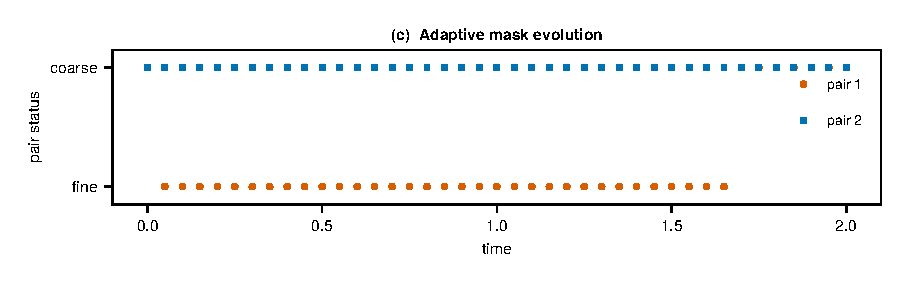
\includegraphics[width=0.8\textwidth]{fig_adaptive_mask}
  \caption{Time-resolved adaptive mask on the $K=4$ Schl\"ogl front. The front
  pair remains at fine resolution while the homogeneous pair is coarsened.}
  \label{fig:adaptive_mask}
\end{figure}

\subsection{Persistent mixed-resolution evolution on an eight-voxel front}

Figure~\ref{fig:k8} shows the main large-grid result. A Schl\"ogl front on a
$K=8$ grid is evolved directly on the mixed-resolution state space. The coarse
marginal $\bar n_2 = n_3+n_4$ is insufficient to distinguish the two fine
interface configurations, while fine resolution inside the active pair
preserves the interface distribution.

\begin{figure}[t]
  \centering
  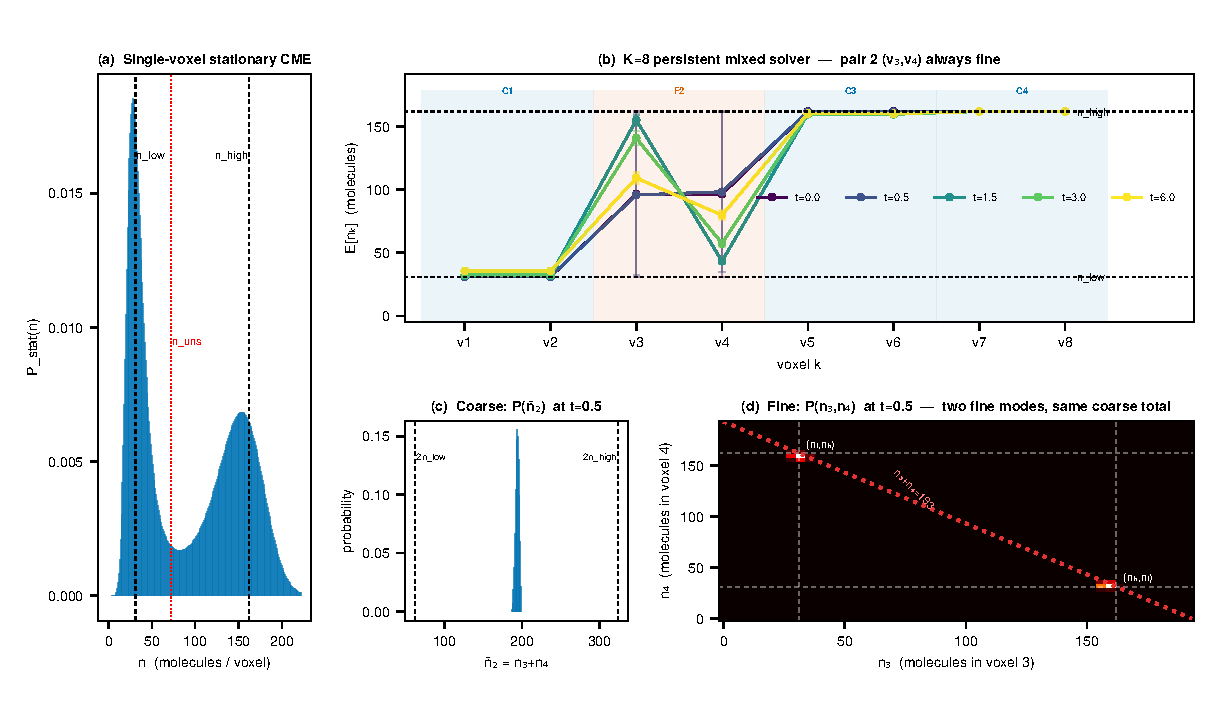
\includegraphics[width=\textwidth]{fig_k8_persistent}
  \caption{$K=8$ mixed-resolution Schl\"ogl front. Pair~2 is retained at fine
  resolution while the surrounding bulk is coarsened. The coarse variable
  $\bar n_2$ cannot distinguish the two fine interface orientations, whereas
  the fine pair distribution resolves them explicitly.}
  \label{fig:k8}
\end{figure}

Figure~\ref{fig:speedup} compares state-space growth in direct and adaptive
coarsened FSP solves, confirming dramatic reduction under coarsening.

\begin{figure}[t]
  \centering
  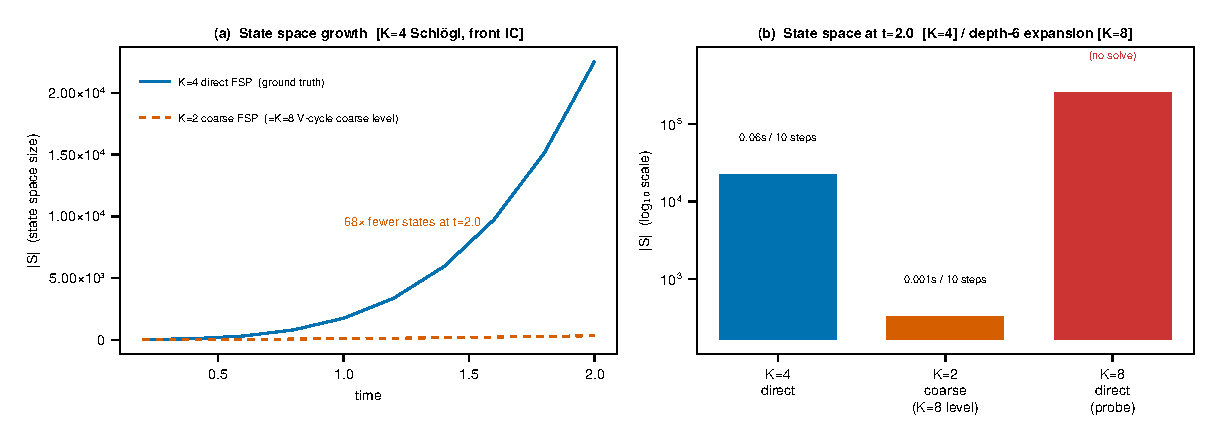
\includegraphics[width=\textwidth]{fig_speedup}
  \caption{State-space reduction under adaptive coarsening on a Schl\"ogl front
  problem.}
  \label{fig:speedup}
\end{figure}

\subsection{FSP versus trajectory sampling on the same mixed model}

Figure~\ref{fig:fsp_ssa} compares direct FSP on a three-dimensional mixed CME
against stochastic simulation of the same mixed generator. The TV distance
between SSA and FSP decays at the expected $N^{-1/2}$ Monte Carlo rate. FSP
returns the full interface distribution directly; trajectory sampling resolves
it only gradually.

\begin{figure}[t]
  \centering
  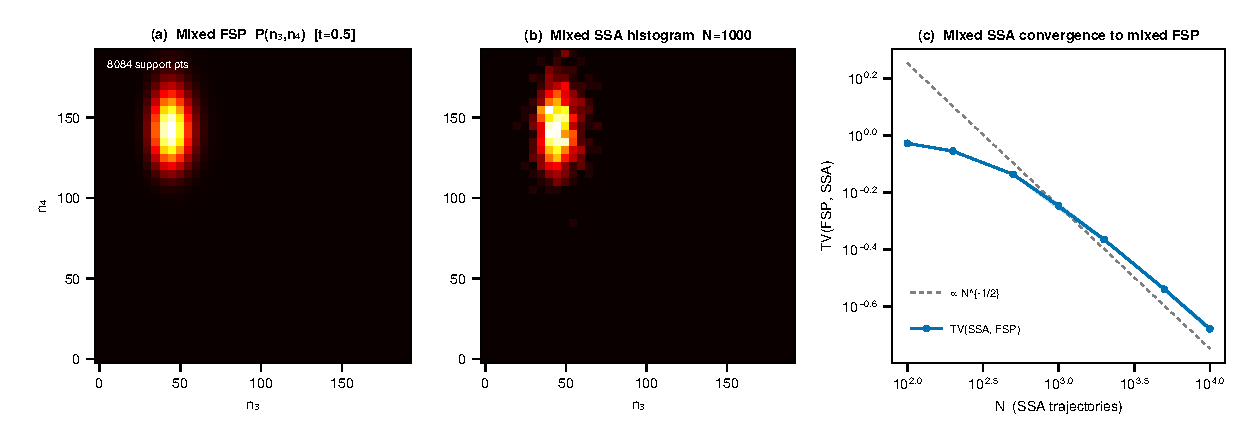
\includegraphics[width=\textwidth]{fig_mixed_fsp_ssa}
  \caption{Mixed FSP versus mixed SSA on the same reduced model. FSP directly
  resolves the interface distribution; SSA converges at the expected Monte Carlo
  rate.}
  \label{fig:fsp_ssa}
\end{figure}

\section{Second-level coarsening and policy validation}
\label{sec:level2}

\subsection{Second-level (quad) coarsening}

The pair-aggregation scheme extends to a second coarsening level by merging
two adjacent level-1 pairs into a single \emph{quad} variable $\tilde n =
\bar n_j + \bar n_{j+1}$, representing four fine voxels with $r=4$
sub-voxels.  The Binomial closure at this level gives
\begin{align*}
  a_{\mathrm{auto}}^{(2)}(\tilde n)
    &= c_1\,\frac{\tilde n(\tilde n-1)}{8}, \\
  a_{\mathrm{rev}}^{(2)}(\tilde n)
    &= c_2\,\frac{\tilde n(\tilde n-1)(\tilde n-2)}{96}.
\end{align*}
Two adjacent level-1 pairs are promoted to a quad only when both satisfy
$\alpha_j^{\mathrm{eff}} < \alpha_{\mathrm{lo2}}$ with $\alpha_{\mathrm{lo2}}
\ll \alpha_{\mathrm{lo}}$. The set of level-2 pairs is therefore always a
subset of the level-1 bulk region, well separated from any front.

\subsection{Isolation test}

With $K=4$ voxels (two pairs), a direct fine FSP is tractable and provides a
reference.  Table~\ref{tab:isolation} shows the TV between the reference
projected onto pair-sum variables and the corresponding coarse distribution, at
$t=0.5$ with voxel spacing $h=1/12$ (matching $K=12$).

\begin{table}[ht]
\centering
\caption{$K=4$ level-2 isolation test at $t=0.5$.  All TV values compare
distributions on the same coarsened variable. The front scenario measures the
catastrophic case excluded by the adaptive policy.}
\label{tab:isolation}
\begin{tabular}{lccc}
\toprule
Scenario & $\TV(p^{\rm fine}\!\downarrow, p^{L1})$ &
           $\TV(p^{\rm fine}\!\downarrow, p^{L2})$ &
           $\TV(p^{L1}\!\downarrow, p^{L2})$ \\
\midrule
Both pairs HIGH (bulk)          & 0.303 & 0.184 & 0.079 \\
Both pairs LOW  (bulk)          & 0.204 & 0.117 & 0.036 \\
Pair~1 LOW, pair~2 HIGH (front) & 0.451 & 0.293 & 0.266 \\
\bottomrule
\end{tabular}
\end{table}

The level-1-vs-level-2 TV (rightmost column) is the intrinsic cost of the
second-level Binomial closure: $0.036$--$0.079$ in bulk, $0.266$ at the front
--- seven times larger.

\subsection{Policy validation}

Table~\ref{tab:policy} reports per-pair diagnostics at $t=0.5$ in the $K=12$
adaptive run.  The effective asymmetry $\alpha_j^{\mathrm{eff}}$ governs level
assignment.

\begin{table}[ht]
\centering
\caption{Per-pair diagnostics at $t=0.5$ in the $K=12$ adaptive run.
Thresholds: $\alpha_{\rm lo}=0.10$, $\alpha_{\rm hi}=0.25$,
$\alpha_{\rm lo2}=0.03$.}
\label{tab:policy}
\begin{tabular}{ccccccl}
\toprule
Pair & Level & $\mu_L$ & $\mu_R$ & $\alpha_j$ & $\alpha_j^{\rm eff}$ & Status \\
\midrule
1 & L1 & 31.0 & 31.0 & 0.000 & 0.003 & bulk \\
2 & L1 & 31.1 & 31.1 & 0.000 & 0.513 & \textbf{front halo}
    ($\beta_{2\to3}=0.51 \gg \alpha_{\rm lo}$) \\
3 & L0 & 96.6 & 97.3 & 0.003 & 0.513 & \textbf{front}
    ($>\alpha_{\rm hi}$, forced fine) \\
4 & L1 & 161.8 & 161.8 & 0.000 & 0.249 & \textbf{front halo}
    ($\beta_{3\to4}=0.25>\alpha_{\rm lo}$) \\
5 & L2 & 162.0 & 162.0 & 0.000 & 0.001 & bulk ($<\alpha_{\rm lo2}$, promoted) \\
6 & L2 & 162.0 & 162.0 & 0.000 & 0.000 & bulk ($<\alpha_{\rm lo2}$, promoted) \\
\bottomrule
\end{tabular}
\end{table}

The inter-pair gradient $\beta$ is the critical protection mechanism.
Pairs~2 and~4 have near-zero internal asymmetry but inherit large
$\alpha^{\mathrm{eff}}$ from the front at pair~3 through $\beta$, blocking
level-2 promotion.  Only pairs~5 and~6, separated from the front by two L1
guards, satisfy $\alpha^{\mathrm{eff}} < \alpha_{\mathrm{lo2}}$ and are
promoted.

The coarse-marginal TV between the level-1 and level-2 runs at $t=0.5$ is
$0.034$, consistent with the bulk regime ($0.036$) in the isolation test.
This confirms the observed approximation cost is the intrinsic cost of the
second-level closure in a homogeneous bulk region, not a front-contamination
artifact.

\section{Discussion}

The present results support four main conclusions.

First, spatial multigrid for the RDME can be formulated as a genuine
probability-generator reduction rather than a heuristic coarsening.
Restriction and prolongation arise naturally from local diffusion
equilibration, the coarse generator is exact in the linear setting, and the
two-level cycle has the complete FAS structure: pre-smooth, restrict, coarse
solve, correct, post-smooth.

Second, the smoother is not an arbitrary component. Intra-pair diffusion acts
precisely on the fast modes introduced by fine-grid spatial discretization.
After pre-smoothing, within-pair distributions are near Binomial and the
restriction operator $\R$ is near-exact. This is what makes the correction
$\delta^{2h} = \tilde p^{2h} - p^{2h}$ small and the V-cycle effective.

Third, the main obstacle in nonlinear bistable systems is not coarsening itself
but coarsening the wrong region. Uniform Binomial prolongation fails at
interfaces because the fine conditional is not near the local equilibrium.
The adaptive strategy resolves this by keeping the active front at fine
resolution and applying coarse closure only in bulk regions where it is
appropriate.

Fourth, the second-level coarsening experiment provides the first evidence that
the policy extends beyond the first coarsening level. The effective asymmetry
$\alpha_j^{\mathrm{eff}}$---including the inter-pair gradient $\beta$ rather
than only the internal $\alpha_j$---produces a protective halo around the
front. Pairs immediately adjacent to the interface have large
$\alpha_j^{\mathrm{eff}}$ even when their internal asymmetry is negligible,
because the front gradient leaks into them through $\beta$. In the $K=12$
test, level-2 coarsening is confined to regions spatially distant from the
active front, where the bulk Binomial closure at $r=4$ introduces $3$--$8\%$
TV error. Whether the same gradient criterion remains sufficient beyond level
2, or for more complex front geometries, is an open question.

The present work has limitations. The most important unresolved issue is state
growth in the mixed FSP when several coarse directions become dynamically
broad; systematic per-coordinate truncation control is a natural next step.
Richer closures for coarse reaction terms at higher coarsening levels, and
extension to multi-species and two-dimensional domains, remain open.

\section{Conclusion}

We have presented a two-level multigrid FSP method for the RDME based on
spatial aggregation of adjacent voxels. The aggregation is a Kemeny--Snell
lumping driven by fast intra-pair diffusion, yielding a probabilistic
restriction--prolongation pair and a Galerkin coarse generator. The two-level
cycle uses intra-pair diffusion as the smoother, exact marginalization as
restriction, a coarse RDME solve, and prolongation of the signed coarse
correction. This construction is exact for linear birth--death--diffusion
systems and provides a tractable FAS-style cycle for nonlinear systems.

In bistable Schl\"ogl front problems, the cycle is accurate in homogeneous
bulk and fails at interfaces; this motivates adaptive mixed-resolution
evolution, which retains fine resolution only where the distribution contains
nonredundant spatial structure. Second-level quad-coarsening extends the
hierarchy one level, and the $K=12$ policy audit shows empirically that the
adaptive $\alpha^{\mathrm{eff}}$ criterion confines it to bulk pairs in this
setting, so the observed coarse-marginal TV is the intrinsic cost of the bulk
closure rather than a front artifact. The resulting method
resolves interface distributions, reduces state-space dimension, and provides
stiffness relief, all within the FSP framework.

\bibliographystyle{plainnat}
\bibliography{references}

\end{document}
